\documentclass[12pt, letterpaper]{article}

\usepackage[utf8]{inputenc}  % Basic character encoding
\usepackage{amsmath}         % For mathematical  formulas
\usepackage{amssymb}         % Provides an extended symbol collection.
\usepackage{mathtools}
\usepackage{pgfplots}        % For plotting
\setcounter{secnumdepth}{0}  % sections are level 1

% Personal data
\title{Pre-Calculus from Zero}
\author{Basic Pre-Calculus Topics}
\date{Dec 2017}

% Style settings
\setlength\parindent{0pt}

% End of preamble
\begin{document}

\maketitle
\section{Introduction}
The Pythagorean theorem $x^2 + y^2 = z^2$ was proved to be invalid for other 
exponents. Meaning the next equation has no integer solutions:
$$x^n+ y^n = z^n$$
\section{Arithmetic}
\section{Algebra}
\section{Sets}
In mathematics, a set is a collection of distinct objects. A set is also itself
an object. For example, the numbers 2, 4, and 6 are distinct objects when 
considered separately, but when they are considered collectively they form a 
single set of size three, written {2,4,6}.
\\
$\mathbb{P}$, denoting the set of all primes:
$\mathbb{P}$ = (2, 3, 5, 7, 11, 13, 17, ...)
\\\\
A prime number is a natural number greater than 1 that has no positive
divisors other than 1 and itself.
\\
$\mathbb{N}$, denoting the set of all natural numbers:
$\mathbb{N}$ = (0, 1, 2, 3, ...)
\\\\
The natural numbers are those used for counting.
\\
$\mathbb{Z}$, denoting the set of all integers: 
$\mathbb{Z}$ = (..., -2, -1, 0, 1, 2, ...)
\\\\
An integer is a number that can be written without a fractional component.
For example, 22, 6, 0 and -2048 are integers,
while 4.75, 5$\frac{1}{2}$ and $\sqrt{2}$ are not.
\\
$\mathbb{Q}$, denoting the set of all rational numbers:
$\mathbb{Q}$ = (a/b : a, b $\in$ Z, b $\neq$ 0)
\\\\
A rational number is any number that can be expressed as the quotient or
fraction p/q of two integers, a numerator p and a non-zero denominator q.
\\
$\mathbb{R}$, denoting the set of all real numbers.
\\\\
A real number is a value that represents a quantity along a line.
\\
\section{Rectangular Coordinates}
Just as you can represent real numbers by points on a real number line, you can
represent ordered pairs of real numbers by points in a plane called the
rectangular coordinate system, or the Cartesian plane, named after the French
mathematician René Descartes (1596–1650).
\\
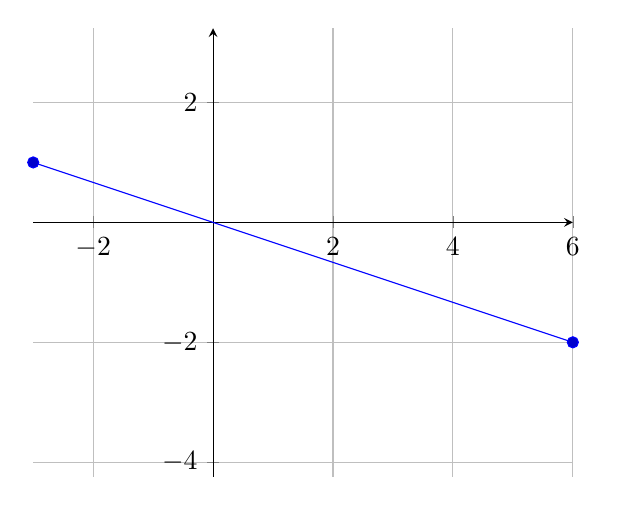
\begin{tikzpicture}
\begin{axis}[axis lines=middle,axis equal,grid=both]
\addplot coordinates{(-3,1) (6,-2)};
\end{axis}
\end{tikzpicture}

\section{Factoring}

The GCF (greatest common factor) of two or more monomials is the product of all 
their common prime factors. For example, the GCF of $6x$ and $4x^2$ is $2x$.
i
For example, to factor $-\frac{3}{5}z^3 - 6z^2$, we would first get a common
denominator and factor as: 
\[ -\frac{3}{5}z^3 - 6z^2 = \frac{-3z^3 - 30z^2}{5} =
\frac{-3z^2(z + 10)}{5} = -\frac{3z^2(z + 10)}{5}\]

\section{Polynomial Functions}

Info here. Add some information on the subject above. 

\section{Rational Functions}

Info here. Add some information on the subject above. 

\section{Exponential Functions}

Info here. Add some information on the subject above. 

\section{Logarythmic Functions}

Info here. Add some information on the subject above. 

\section{Trigonometry}

Info here. Add some information on the subject above. 

\section{Analytic Trigonoetry}

Info here. Add some information on the subject above. 


% Sample Exam /////////////////////////////////////////////////////////////////
\section{Sample Final Exam}
Below is a sample final exam:

% DONE PASS 1
% Question 01 /////////////////////////////////////////////////////////////////
\subsection{Question 1:}
1. Let $f(x)=x-7$ and let $g(x)=x^2-49$. Specify the domain of $f(x)/g(x)$.\\\\
Notes: The domain is the set of all possible x-values which will make the 
function "work", and will output real y-values. The domain of an arithmetic 
combination of functions is all real numbers that are common to the 
domains. \\

Rules to remember:
\begin{enumerate}
  \item The denominator (bottom) of a fraction cannot be zero.
  \item The number under a square root sign should be positive.
\end{enumerate}

Step-by-Step Solution:
\begin{enumerate}
  \item The domain of $f(x)=x-7$ is all real number 
  $\mathbb{R}$ (-$\infty$, $\infty$). 
  \item The domain of $g(x)=x^2-49$ is all real number 
  $\mathbb{R}$ (-$\infty$, $\infty$).
  \item \textbf{Answer:} all real number $\mathbb{R}$ (-$\infty$, $\infty$).
\end{enumerate}

Book Notes:
\begin{enumerate}
  \item Read 1.8 -- Combinations of Functions, Page 84
    \item Read 1.8 --Finding the Domains of Quotients of Functions, Page 85  
\end{enumerate}

% TODO
% Question 02 /////////////////////////////////////////////////////////////////
\subsection{Question 2:}
2. Draw the graph of $y=2cos(2x)$ from $x=0$ to $x=2\pi$.

\newpage
% TODO Cant figure out how to make a plot for this.
% Question 03 /////////////////////////////////////////////////////////////////
\subsection{Question 3:}
3. Draw the graph of $y=2-|x-5|$.
\\\\\\\\\\

% TODO
% Question 04 /////////////////////////////////////////////////////////////////
\subsection{Question 4:}
Write an equation of the line parallel to the line 
  $y=2-\frac{3}{2}x$ at $(4,-2)$ and sketch its graph.
  \\\\
  Rules to remember:
  \begin{enumerate}
    \item Take the negative reciprical for the slope.
    \item The number under a square root sign should be positive.
  \end{enumerate}

% TODO
% Question 05 /////////////////////////////////////////////////////////////////
\subsection{Question 5:}
  Draw the graph of $y=2x^2-16x+24$ and label its minimum.
  \\\\
  Rules to remember:
  \begin{enumerate}
    \item Take the negative reciprical for the slope.
    \item The number under a square root sign should be positive.
  \end{enumerate}

% TODO
% Question 06 /////////////////////////////////////////////////////////////////
\subsection{Question 6:}
  Draw the graph of $y=\sqrt{x-7}$.
  \\\\

  Rules to remember:
  \begin{enumerate}
    \item Take the negative reciprical for the slope.
    \item The number under a square root sign should be positive.
  \end{enumerate}

% Question 07 /////////////////////////////////////////////////////////////////
\subsection{Question 7:}
  In the triangle $ABC$, side $a=5in.$, side $b=10in.$ and $\angle C=60^\circ$.
  Find the length of side $c$. (Leave your answer in radical form.) 
  \\\\
  Rules to remember:
  \begin{enumerate}
    \item Take the negative reciprical for the slope.
    \item The number under a square root sign should be positive.
  \end{enumerate}

% Question 08 /////////////////////////////////////////////////////////////////
\subsection{Question 8:}
  Write an equation of the line given the graph in Figure A:
  \\\\
  Rules to remember:
  \begin{enumerate}
    \item Take the negative reciprical for the slope.
    \item The number under a square root sign should be positive.
  \end{enumerate}

% Question 09 /////////////////////////////////////////////////////////////////
\subsection{Question 9:}
  Write an equation of the parabola given in the graph in Figure B. 
  \\\\
  Rules to remember:
  \begin{enumerate}
    \item Take the negative reciprical for the slope.
    \item The number under a square root sign should be positive.
  \end{enumerate}

% Question 10 /////////////////////////////////////////////////////////////////
\subsection{Question 10:}
  Let $g(x)=18e^{0.07x}$. Write the inverse of $g$ and specify its domain.
  \\\\
  Rules to remember:
  \begin{enumerate}
    \item Take the negative reciprical for the slope.
    \item The number under a square root sign should be positive.
  \end{enumerate}

% Question 11 /////////////////////////////////////////////////////////////////
\subsection{Question 1:}
  Let $f(x)=15x-1$. Compute and simplify the difference quotient given by:
  $$\frac{f(x+h)-f(x)}{h}$$
  \\\\
  Rules to remember:
  \begin{enumerate}
    \item Take the negative reciprical for the slope.

    \item The number under a square root sign should be positive.
  \end{enumerate}

% Question 12 /////////////////////////////////////////////////////////////////
\subsection{Question 12:}
  If $sin(x) = -3/5$ and $x$ is and angle in Quadrant $III$, 
  find the value of tan(x). 
  \\\\
  Rules to remember:
  \begin{enumerate}
    \item Take the negative reciprical for the slope.
    \item The number under a square root sign should be positive.
  \end{enumerate}

% Question 13 /////////////////////////////////////////////////////////////////
\subsection{Question 13:}
  State the formula for $sin(a+b)$ and use it to show $sin(a+3\pi/2)=-cos(a)$.
  \\\\
  Rules to remember:
  \begin{enumerate}
    \item Take the negative reciprical for the slope.
    \item The number under a square root sign should be positive.
  \end{enumerate}

% Question 14 /////////////////////////////////////////////////////////////////
\subsection{Question 14:}
  Draw the graph of $f(x)=\frac{2}{9-x^2}$. Indicate asymptotes.
  \\\\
  Rules to remember:
  \begin{enumerate}
    \item Take the negative reciprical for the slope.
    \item The number under a square root sign should be positive.
  \end{enumerate}

% Question 15 /////////////////////////////////////////////////////////////////
\subsection{Question 15:}
  Draw the graph of:
  \[F(x) =
    % Start pepiecewise function
    \begin{cases}
        \text{$8-4x$,} & \text{for $x\le 5$} \\
        \text{$4x-8$,} & \text{for $x>5$}
    \end{cases}\]

% Question 16 /////////////////////////////////////////////////////////////////
\subsection{Question 16:}
When a vendor prices key chains at \$5 each, she sells 210 key chains. For each \$1 she raises the price, she sells ten fewer key chains. USE AN EQUATION to determine what she should charge to maximize her revenue from sales..
  \\\\

  Rules to remember:
  \begin{enumerate}
    \item Take the negative reciprical for the slope.
    \item The number under a square root sign should be positive.
  \end{enumerate}

% Question 17 /////////////////////////////////////////////////////////////////
\subsection{Question 17:}
The population North Oblivion is now 1400 people and is known to double every 12 years.
  \\\\
 
  Rules to remember:
  \begin{enumerate}
      \item (a). Write a function that gives the population, $P(t)$, after $t$ years.
      \item (b). How many years will it take for the population to reach 4200? 
        (a formula will suffice.)
  \end{enumerate}

\end{document}
